\begin{Exercise}[title=Détente de Joule-Thomson]
		Un gaz à pour équation d'état $P(V-nb)=nRT$ et son énergie interne obéit à la première loi de joule $C_{vm} = 2,5R$ et $C_{p_m}=3,5 R$ .
		\Question
		\subQuestion Préciser les unités de $R$ et $b$.
		\subQuestion Déterminer l'expression de l'enthalpie molaire de ce gaz en fonction de $R,b$ et $T$.
		\emph{une mole de ce gaz subit une détente de Joule-Thomson: Cette détente consiste en la lente détente d'un gaz à travers un tube très fin et isolé thermiquement qui fait passer sa pression de $P_1$ à $P_2$ en régime permanent.}
		\Question
		\subQuestion Faire un schéma.
		\subQuestion Calculer le travail des forces de pression lors de cette transformation.
		\subQuestion Montrer que l'enthalpie du gaz est conservée.
		\subQuestion On mesure les températures correspondantes $T_1$ et $T_2$ montrer que ce dispositif permet de mesurer $b$.
\end{Exercise}
\begin{Answer}
		\Question
		\subQuestion $R$ est en \si{\J\per\K\per\mole} et $b$ \si{\m^3\per\mole}.
		\subQuestion $H_m = U_m + pV_m = C_{V_m} T + RT  + pb$. le gaz ne suit pas la deuxième loi de joule.
		\Question
		\subQuestion Avec S une surface de petite taille.
		\begin{center}
			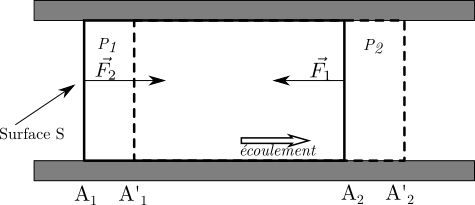
\includegraphics[width = 0.5\linewidth]{../fig/joule-thomson.png}
		\end{center}
		\subQuestion Avec  le premier principe : $\Delta U = W = p_1 V_1 - p_2 V_2$.  on note $U_1$ (respectivement $U_2$) l'énergie interne du fluide  compris entre $A_1$ et $A_1'$ (respectivement $A_2$ et $A_2'$) et $U_c$ l'énergie interne de la partie commune on a :
		\[ U_2+U_c -(U_1+U_c) = p_1dV_1 -p_2dV_2 \implies H_2=H_1\] .L'enthalpie du gaz est conservée.
		\subQuestion $b=\frac{(C_{v_m}+R)(T_2-T_1)}{p_1-p_2}$
\end{Answer}
